\documentclass[oneside,12pt]{article}

\usepackage{amsmath,amsfonts}
\usepackage{graphicx}

\begin{document}
	
	\section*{MAS2806-PHY2039 Assessment 1 plotting mark scheme}
	
	\noindent\textbf{Question 1 or 2 (depending on randomisation)}
	
	\begin{minipage}{0.49\textwidth}
		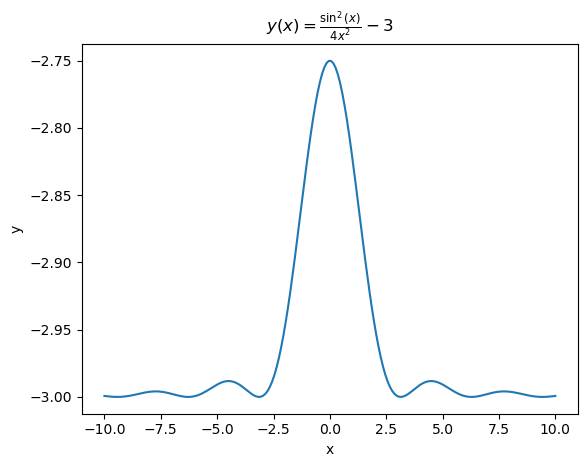
\includegraphics[scale=0.65]{q1.png}
	\end{minipage}
	\begin{minipage}{0.49\textwidth}
		\begin{itemize}
			\item Maximum mark: \(8\).
			\item \(4\) marks for graph of a similar function to that in the model solution. If graph is not sufficiently smooth (e.g. it appears jagged) deduct \(1\) mark.
			\item \(2\) marks for reasonable ranges of variables. E.g. if \(y\) is too big to fully display behaviour of the function deduct \(1\) mark.
			\item \(1\) mark for \(x\), \(y\) labels on axes.
			\item \(1\) mark for appropriate labelling of function in plot title, legend, or equivalent. The label does not have to be typeset in \LaTeX (as on the left) e.g. \verb|sin^2(x)/(4x^2) - 3| is sufficient.
		\end{itemize}
	\end{minipage}
	
	\vspace*{15pt}
	\hrule height 1pt
		
	\noindent\textbf{Question 4}
	
	\begin{minipage}{0.49\textwidth}
		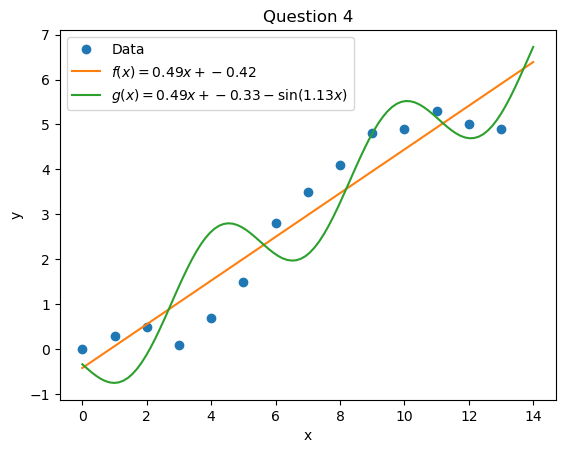
\includegraphics[scale=0.65]{q4.png}
	\end{minipage}
	\begin{minipage}{0.49\textwidth}
		\begin{itemize}
			\item Maximum mark: \(8\).
			\item \(1\) mark for data plotted as points.
			\item \(1\) mark for a line of best fit (orange on left).
			\item \(2\) marks for a fitted function reasonably similar to the green curve on the left. Deduct \(1\) mark is the curve is not sufficiently smooth.
			\item \(2\) marks for reasonable ranges of variables and labels on axes.
			\item \(2\) marks for appropriate labelling of functions in a legend. The labels do not have to be typeset in \LaTeX (as on the left) e.g. \verb|a*x+b| is sufficient. Deduct \(1\) mark if a function is missing, deduct \(2\) marks if two are missing.
		\end{itemize}
	\end{minipage}
	
	\newpage
	
	\noindent\textbf{Question 5 part d}
	
	\begin{minipage}{0.49\textwidth}
		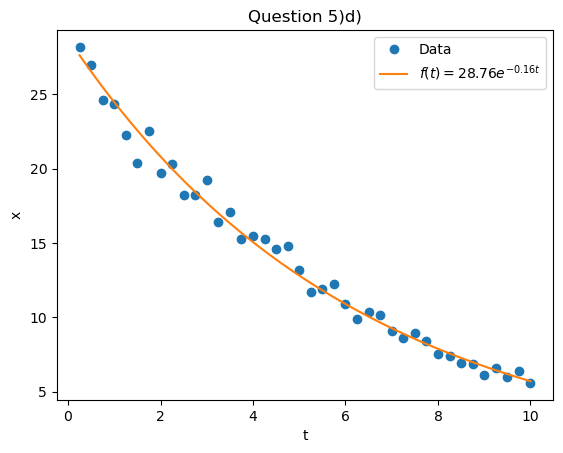
\includegraphics[scale=0.65]{q5d.png}
	\end{minipage}
	\begin{minipage}{0.49\textwidth}
		\begin{itemize}
			\item Maximum mark: \(10\).
			\item \(1\) mark for data plotted as points.
			\item \(4\) marks for a fitted function reasonably similar to the orange curve on the left. Deduct \(1\) mark if the curve is not sufficiently smooth. Deduct \(1\) mark if the curve appears to be a straight line.
			\item \(1\) mark for linear axes e.g. clear from axis labels that scale is linear.
			\item \(2\) marks for reasonable ranges of variables and labels on axes.
			\item \(2\) marks for appropriate labelling of functions in a legend. The labels do not have to be typeset in \LaTeX (as on the left) e.g. \verb|ae^(bt)| is sufficient. Deduct \(1\) mark if a function is missing, deduct \(2\) marks if two are missing.
		\end{itemize}
	\end{minipage}
	
	\vspace*{15pt}
	\hrule height 1pt
	
	\noindent\textbf{Question 5 part e}
	
	\begin{minipage}{0.49\textwidth}
		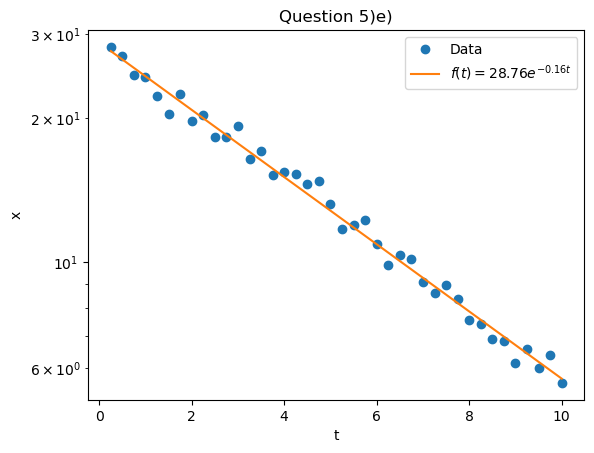
\includegraphics[scale=0.65]{q5e.png}
	\end{minipage}
	\begin{minipage}{0.49\textwidth}
		\begin{itemize}
			\item Maximum mark: \(10\).
			\item \(1\) mark for data plotted as points.
			\item \(4\) marks for a fitted function reasonably similar to the orange line on the left. Deduct \(1\) mark if the line does not appear to be a straight.
			\item \(1\) mark for semilogarithmic axes e.g. clear from axis labels that dependent variable is on a logarithmic scale.
			\item \(2\) marks for reasonable ranges of variables and labels on axes.
			\item \(2\) marks for appropriate labelling of functions in a legend. The labels do not have to be typeset in \LaTeX (as on the left) e.g. \verb|ae^(bt)| is sufficient. Deduct \(1\) mark if a function is missing, deduct \(2\) marks if two are missing.
		\end{itemize}
	\end{minipage}
	
	
	
	
	

\end{document}